% !TeX root = ../../thesis.tex

Our main result is the tool we developed that we are going to further explore its components. The main one is the Bayesian network developed, and its structure is presented in figure \ref{fig:network}. The example in the image shows the probability for all the classes in the category of Robson group, taking into account the values of the other categories (both known and unknown). In this case, the probability for Robson group number 3 is 77.41\%. 
%TC:ignore
\begin{figure}[h!]
    \centering
    \caption{Bayesian Network learned. Nodes acronyms are explained in appendix 1. The example shows the inference for the Robson Group (10 categories) and the probability of each category, given a set of other features.} \label{fig:network} 
    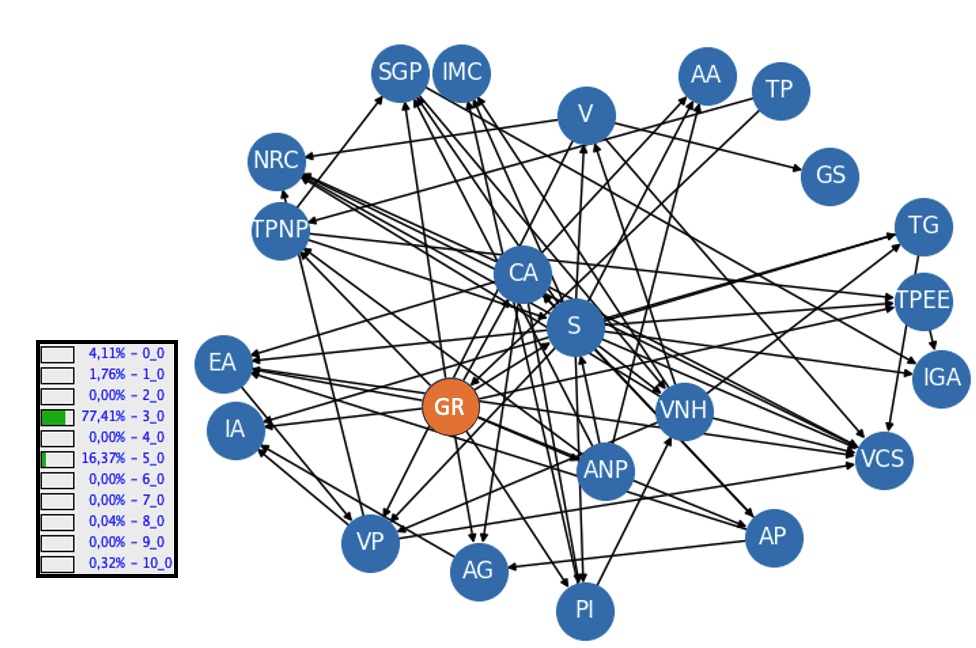
\includegraphics[scale=0.38]{figures/new-bn.png}
\end{figure}
    %TC:endignore

The results of the cross validation can be seen in the table \ref{tab:result_auc}. The average \ac{auroc} was 0.857. In parentheses is the number of non-null rows that were used in the validation for that column as target.


\begin{table}[h!]
    \caption{Repeated Cross-Validation (10x2) Results: Column description with \ac{auroc} along with 95\% CI. (n) is the number of non null rows.} \label{tab:result_auc} 
   
   \renewcommand{\arraystretch}{1.2}
   %\setlength{\tabcolsep}{8pt}
   \centering
   \begin{tabular} {lcc }
    \toprule
    Name of Variable (n) &               Average &               95\% CI \\
 \midrule
   Nr of previously born babies (44387) & 0.944 & [0.943, 0.945] \\
   Nr pregnancies (73335) & 0.797 & [0.778, 0.816] \\
   Nr eutotic deliveries (28809) & 0.969 & [0.968, 0.969] \\
   Nr Prev. C-section (17879)& 0.958 & [0.958, 0.958] \\
   Mother’s Age (73337) & 0.638 & [0.637, 0.638] \\
   Mother’s weight start (63324)& 0.881 & [0.88, 0.881] \\
   BMI (62260) & 0.881 & [0.881, 0.882] \\
   Nr Prenatal Consultations (61388) & 0.75 & [0.75, 0.75] \\
   Nr Weeks on admission (72715) & 0.968 & [0.968, 0.969] \\
   Pregnancy weeks on delivery (73217) & 0.974 & [0.974, 0.974] \\
   Nr deliveries with vacuum (15985) & 0.974 & [0.974, 0.974] \\
   Pregnancy Type (64517) & 0.728 & [0.726, 0.73]\\
   If pregnancy was accompanied in the hospital (49738)& 0.894 & [0.893, 0.895] \\
    If delivery was spontaneous (26360) & 0.816 & [0.815, 0.816] \\
    Baby’s position admission (20166)& 0.751 & [0.743, 0.758] \\
    Robson Group (69280) & 0.931 & [0.93, 0.932] \\
    If pregnancy was accompanied (73219) & 0.983 & [0.982, 0.983] \\
    Delivery Type (73350)& 0.866 & [0.865, 0.868] \\
    If was accompanied in the primary care setting (49812) & 0.79 & [0.789, 0.791] \\
    Baby’s position delivery (73227) & 0.942 & [0.938, 0.946] \\
    Blood Group (73132) & 0.514 & [0.507, 0.52] \\
    Hospital ID (73352) & 0.896 & [0.896, 0.897] \\
    If accompanied in a private care setting (18049) & 0.771 & [0.77, 0.772] \\
    Actual Type of delivery (65606) & 0.952 & [0.951, 0.952] \\
   \hline
    \multicolumn{3}{c}{\textbf{Average}  \textbf{0.857 [0.846, 0.868]}} \\
   
   \hline
   \end{tabular}
   \end{table}

\subsection{Deployment \& Validation}

The purpose of this model is to serve as an \ac{api} for usage within a healthcare institution and act as a supplementary data quality assessment tool. Although a concrete, vendor-specific information model and health information system were initially used, our goal is to develop a more universal clinical decision support system. This system should be usable across all systems involved in birth and obstetrics departments. Therefore, we constructed it using the \ac{hl7} \ac{fhir} R5 version standard. This approach simplifies the process of \ac{api} interaction. Rather than utilizing a proprietary model for the data, we based our decision on the use of \ac{fhir} resources: \textit{Bundle} and \textit{Observation}. These resources handle the request and response through a customized operation named "\$quality\_check". We intend to publish the profiles of these objects to streamline \ac{api} access via standardized mechanisms and data models. The model then makes use of the customized operation and of several base resources to construct a \ac{fhir} message, which are: \textit{Bundle}, \textit{MessageHeader}, \textit{Observation}, \textit{Device}. \textit{Observation} is where the information about the record is contained, Device contains information about the model, and \textit{MessageHeader} is used to add information about the request. Finally, the Bundle is used to group all of these resources together. The current version of the profiles can be accessed here\unskip~\cite{almeidaObstetricsClinicalDecision}. 

For validation, we deployed the tool in docker format in a hospital to gather new data. We gathered 3223 new cases and returned a score for quality as exemplified in figure \ref{fig:scores}. Being that the score is from 0 to 1, the average score was 0.75 and \ac{iqr} was 0.016. The formula gives weights to different dimensions since we feel some are more robust than others. We gave more weight to rule system, and gave less to the missing and \ac{iqr} score.

As for the clinicians' assessment, we got 4 answers. Figure \ref{fig:clinical-dq} shows the distribution of the perceived ranking of each record.


%TC:ignore
\begin{figure}[htbp]
\centering
\caption{Model score for newly seen data}\label{fig:scores} 
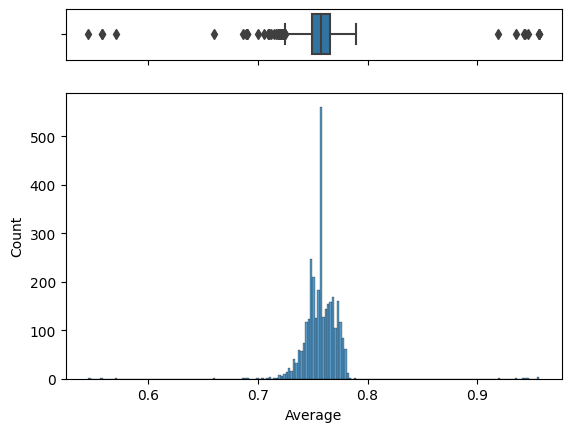
\includegraphics[scale=0.78]{figures/Scoring_V2.png}
\end{figure}
%TC:endignore

%TC:ignore
\begin{figure}[htbp]
\centering
\caption{Distribution of rankings obtained from the assessment of 10 records by 4 different clinicians. Y is the distribution of clinicians' assessment, X is the patient ID.}\label{fig:clinical-dq} 
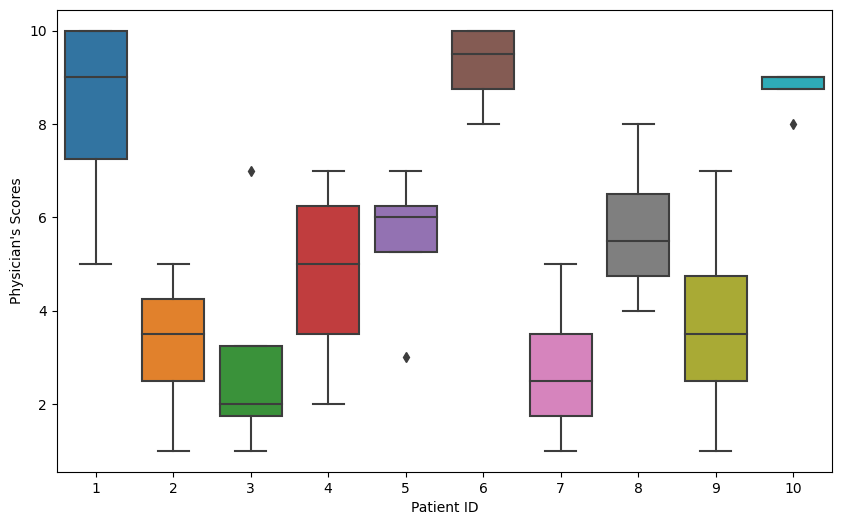
\includegraphics[scale=0.52]{figures/clinical_assessment_no_model.png}
\end{figure}
%TC:endignore

Figure \ref{fig:auc_changes} shows the performance of the model with several ranking thresholds to differentiate bad quality record from good quality record. Each line/color is a threshold (3,4,5,6) and the \ac{auroc} is shown in the label. The Average \textit{Spearman's} Rank Correlation Coefficient was 0.42 (\textit{P}=.23) and the Kendall's Tau was 0.3 (\textit{P}=.2). Both tests were based on an $\alpha$ of 0.05.

%TC:ignore
\begin{figure}[htbp]
    \centering
    \caption{Model Performance in terms of \ac{auroc}, depending on the threshold defined on the physician assessed data. The colours show different threshold used to consider a bad quality record given the average ranking. Label shows the threshold and respective \ac{auroc}.}\label{fig:auc_changes} 
    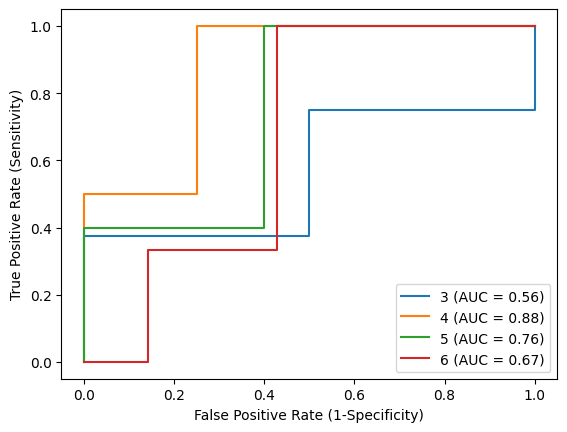
\includegraphics[scale=0.78]{figures/auroc_curve_threshold.png}
    \end{figure}
    %TC:endignore